\documentclass[12pt,a4paper]{article}
\usepackage[left=30mm, right = 30mm, top = 30mm, bottom = 30mm]{geometry}

%************** FONT **************
\usepackage[LGR,T1]{fontenc}
\usepackage[scaled=0.88]{beraserif}
\usepackage[scaled=0.85]{berasans}
\usepackage[scaled=0.84]{beramono}
\usepackage{mathpazo}
\usepackage[T1,euler-digits]{eulervm}

%************ GREY BOX ************
\usepackage[dvipsnames]{xcolor}
\usepackage[framemethod=default]{mdframed}
\global\mdfdefinestyle{greybox}{%
     linecolor=gray!20,linewidth=0.15cm,backgroundcolor=gray!20,%
     %leftmargin=-0.5cm,rightmargin=-0.5cm, 
     innerleftmargin=0.4cm,innerrightmargin=0.4cm
}

%************ Other ************
\usepackage{amsmath} % equations
\usepackage{graphicx}
\usepackage{booktabs}
\usepackage[colorlinks=true,urlcolor=redBurn,linkcolor=blue]{hyperref}
\usepackage[utf8]{inputenc}
%\usepackage{titlesec}

% left align title, author, and date
%\makeatletter
%\renewcommand{\maketitle}{\bgroup
%  \flushleft{\huge{\textbf{\@title}}}  \vspace{5mm}
%    \setlength{\parindent}{22pt}
  
%  \large{\@author} 	\\\vspace{1.5mm}
%  \large{\today}
%\egroup
%}
%\makeatother
\usepackage{titling}
\pretitle{\begin{center}\huge\textbf} 
\posttitle{\end{center}}
%\preauthor{\begin{flushleft}\large} 
%\postauthor{\end{flushleft}}
%\predate{\begin{flushleft}\large} 
%\postdate{\end{flushleft}}

%******* Title, author, date *********
\title{A Journey to the West}
\author{Miao Cai}
\date{\today}

%************ MAIN ************
\begin{document}
\maketitle

\section{Introduction}
\begin{mdframed}[style=greybox] 
Don't practice until you get it right, practice until you can't get it wrong.
\flushright{--- Some coach}
\end{mdframed}

The authors would like to thank the reviewers for their comments, which significantly helped improving the manuscript. We believe we have addressed all the issues raised in the following rebuttal. For each comment, we have first highlighted the issue, then we provided an answer, and finally we described how the manuscript was adjusted.



\section{Methods}
Copy-paste the new version of the text in the manuscript here. Don't hesitate to put the new figures and all other modifications you have introduced in the manuscript as a result of the comment. It is important to make it very easy for the reviewer to check the implementation. In very exceptional case, you might just refer to a section number but I would advise against that.

The authors would like to thank the reviewers for their comments, which significantly helped improving the manuscript. We believe we have addressed all the issues raised in the following rebuttal. For each comment, we have first highlighted the issue, then we provided an answer, and finally we described how the manuscript was adjusted.
\begin{align}
\begin{split}
Y_i &\sim \text{Bernoulli}(p_i)\\	
\log \frac{p_i}{1 - p_i} & = \beta_0 + \beta_1x_1 + \beta_2x_2 + \cdots + \beta_kx_k	
\end{split}
\end{align}

The likelihood function is:

\begin{align}
\begin{split}
L_{i}=& \int \prod_{j=1}^{n_{i}} f\left(y_{i j}\right)\left[h_{0}\left(x_{i}\right) \exp \left(Z_{i}^{T} \alpha+\gamma_{1} a_{i}+\gamma_{2} b_{i}\right)\right]^{\Delta_{i}} \\ 
& \exp \left[-\int_{0}^{x_{i}} \exp \left(Z_{i}^{T} \alpha+\gamma_{1} a_{i}+\gamma_{2} b_{i}\right) h_{0}(t) d t\right] \phi\left(a_{i}, b_{i}\right) d a_{i} d b_{i} 
\end{split}
\end{align}


The authors would like to thank the reviewers for their comments, which significantly helped improving the manuscript. We believe we have addressed all the issues raised in the following rebuttal. For each comment, we have first highlighted the issue, then we provided an answer, and finally we described how the manuscript was adjusted.

\section{Results}
The authors would like to thank the reviewers for their comments, which significantly helped improving the manuscript. We believe we have addressed all the issues raised in the following rebuttal. For each comment, we have first highlighted the issue, then we provided an answer, and finally we described how the manuscript was adjusted.

\begin{figure}
	\center
	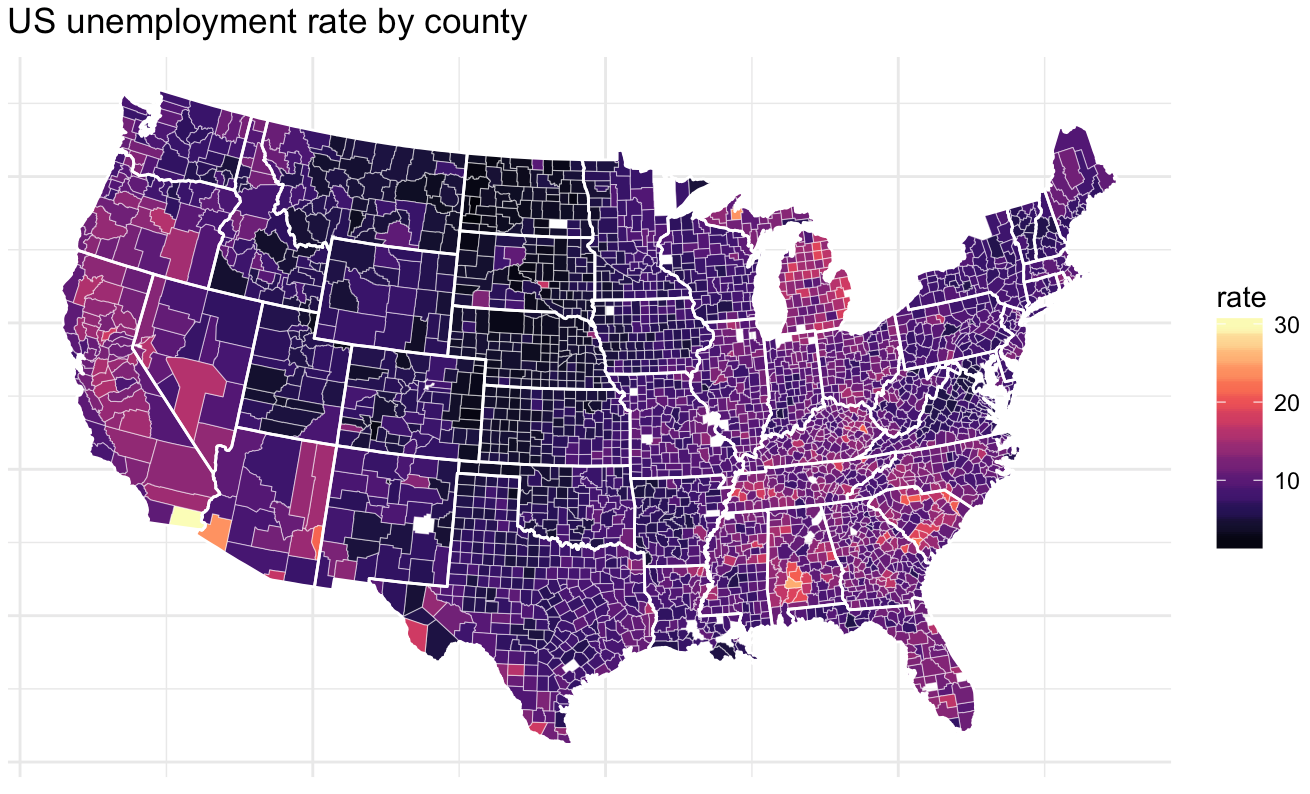
\includegraphics[width=\textwidth]{figs/viridis_map.png}
\end{figure}
The authors would like to thank the reviewers for their comments, which significantly helped improving the manuscript. We believe we have addressed all the issues raised in the following rebuttal. For each comment, we have first highlighted the issue, then we provided an answer, and finally we described how the manuscript was adjusted.

The authors would like to thank the reviewers for their comments, which significantly helped improving the manuscript. We believe we have addressed all the issues raised in the following rebuttal. For each comment, we have first highlighted the issue, then we provided an answer, and finally we described how the manuscript was adjusted.

The authors would like to thank the reviewers for their comments, which significantly helped improving the manuscript. We believe we have addressed all the issues raised in the following rebuttal. For each comment, we have first highlighted the issue, then we provided an answer, and finally we described how the manuscript was adjusted.

\end{document}
